\documentclass[12pt, letterpaper]{article}
\usepackage[ngerman]{babel}
\usepackage{graphicx}
\usepackage{wrapfig}
\usepackage{titlesec}
\usepackage{geometry}
\usepackage[font=scriptsize]{caption}
\usepackage{blindtext}
\usepackage{hyperref}
\usepackage{tabularx}
\usepackage{subcaption}
\usepackage{verbatim}
\usepackage{fancyvrb}
\usepackage{listings}
\usepackage{xcolor}
\usepackage{multirow}
\usepackage{array} % Für die Spaltenbreitenanpassung
\usepackage{booktabs} % Für schönere Tabellen
\usepackage{geometry}
\usepackage{arydshln}
\usepackage{colortbl}
\usepackage{forest}
\usepackage{caption}
\usepackage{pifont}
\usepackage{amssymb}
\usepackage{enumitem}
\renewcommand{\lstlistlistingname}{Programmcode}

\geometry{a4paper, margin=2cm}
\hypersetup{
  colorlinks = true,
  linkcolor = black,
  urlcolor = blue,
}

% \captionsetup{justification=raggedright,singlelinecheck=false}
\geometry{
 a4paper,
 total={170mm,257mm},
 left=20mm,
 top=20mm,
 }
%  \titleformat{\section}[display]
%    {\normalfont\bfseries}{}{0pt}{\huge}

\lstdefinestyle{py}{
    language=Python,
    backgroundcolor=\color{white},
    keywordstyle=\color{blue}\bfseries,        % Default Python keywords
    commentstyle=\color{brown}\bfseries,         % Comments
    stringstyle=\color{brown},                 % Strings
    numberstyle=\tiny\color{gray},             % Line numbers
    basicstyle=\ttfamily\small,                % Base font
    identifierstyle=\color{black},             % Default for variable names
    keywordstyle=[2]\color{cyan},              % Functions
    keywordstyle=[3]\color{purple},            % Types
    breaklines=true,
    showstringspaces=false,
    tabsize=4,
    captionpos=b,
    %numbers=left,
    %numbersep=10pt,
    frame=single
}

% Define specific keywords
\lstset{
    morekeywords={import, from, def, return},  % Default Python keywords
    morekeywords=[2]{print, println, len, range, input}, % Functions
    morekeywords=[3]{int, float, str, list, dict, bool} % Types
}


\lstdefinestyle{cpp}{
    language=C,
    backgroundcolor=\color{white},
    keywordstyle=\color{blue}\bfseries,        % Standard Keywords
    commentstyle=\color{green}\itshape,        % Kommentare
    stringstyle=\color{orange},                % Strings
    numberstyle=\tiny\color{gray},             % Zeilennummern
    basicstyle=\ttfamily\small,                % Basis-Schriftart
    identifierstyle=\color{black},             % Standard für Variablennamen
    keywordstyle=[2]\color{cyan},              % Funktionen
    keywordstyle=[3]\color{purple},            % Typen
    breaklines=true,
    showstringspaces=false,
    tabsize=4,
    captionpos=b,
    %numbers=left,
    %numbersep=10pt,
    frame=single
}

% Spezifische Keywords definieren
\lstset{
    morekeywords={if, else, while, return},         % Standard C-Keywords
    morekeywords=[2]{printf, scanf, main, malloc},  % Funktionen (inkl. malloc)
    morekeywords=[3]{int, float, char, double}      % Typen
}

%\lstset{style=pycharm-light}

  
\usepackage{lipsum}  
\graphicspath{ {./Bilder/} }
\author{Oleksii Baida}
\date{Mai 2024}
\begin{document}
\begin{titlepage}
  
\includegraphics[width = 0.25\pdfpagewidth]{./Bilder/FHDO.jpg}
  \begin{center}
    
    \huge \textbf{\textsf{Bachelorarbeit}} \\
    \vspace{3cm}
    \large \textbf{Oleksii Baida}\\
    \textbf{Matrikelnummer 7210384}\\
    \vspace{3cm}
    \large \textbf{Sicherheits- \& Steuerungssytem für das Haus}\\
    \vspace{1cm}
    \large \textbf{Bericht}\\
    \vspace{1cm}
    \today
  \end{center}
\end{titlepage}

\tableofcontents
\pagebreak

\section{Einleitung}
\par In einer Welt, die zunehmend von vernetzten Geräten und dem Internet der Dinge geprägt ist, wird die Entwicklung effizienter und benutzerfreundlicher Systeme zur Steuerung und Überwachung von Gebäuden immer relevanter. Im Jahr 2024 wurde in Deutschland die Anzahl von über 19 Millionen Haushalten, die ein oder mehrere smarte Geräte besaßen, verzeichnet. Es wird prognostiziert, dass sich diese Zahl innerhalb der nächsten drei Jahre verdoppeln wird \cite{statita_smhomes}.
\par Moderne Steuerungs- und Sicherheitssysteme tragen zur Effizienzsteigerung und Ressourcenschonung bei. Laut Günther Ohland, Vorstandsmitglied des Branchenverbands "Smarthome Initiative Deutschland", ermöglichen diese Systeme eine Reduktion des Heizenergieverbrauchs um 20 bis 30 Prozent \cite{spiegel_heizung}. Die Kosten für die smarte Technik rechnen sich in der Regel nach zwei Jahren. Die Systeme übernehmen ein Teil der täglichen Aufgaben, wie das Ein- und Ausschalten des Lichts, die Reglung der Raumtemperatur oder das Aufräumen des Hauses etc. Der Aufgabenbereich der Systeme ist dabei nur nach den Bedürfnissen der Benutzerinnen und Benutzer abgegrenzt.
\par Im Rahmen meiner Bachelorarbeit wird ein System zur Steuerung und Überwachung des Hauses entwickelt. Das Ziel dieser Arbeit ist die Erstellung einer Schnittstelle, die die Interaktion des Benutzers mit den Geräten in seinem Haushalt ermöglicht und den Benutzer über gefährliche Vorgänge in seinem Haus informiert. 
\par Im Rahmen der Entwicklung dieses Systems wurden die aktuellen Technologien zur Erstellung eines Webinterfaces und zur Kommunikation zwischen den Geräten eingesetzt. \textbf{TODO Kurz erklären was in Kapitel 2,3,4,5 ... erklärt wird}

\newpage
\section{Grundlagen \& Theorie}
\par In diesem Abschnitt erfolgt die detaillierte Darstellung der technischen Informationen zu den verwendeten Komponenten und Technologien. 
  \subsection{Hardware}
    \subsubsection{Arduino}
    \subsubsection{ESP8266}
    \subsubsection{Raspberry Pi}
    \subsubsection{ESP32}
    \subsubsection{M5Stick}
    \subsubsection{BME680}
    \subsubsection{VCNL}
    

  \subsection{Kommunikationsprotokolle}
  \subsubsection{HTTP}
  \subsubsection{MQTT}
  \subsubsection{UART}
  \subsubsection{I2C}
    
  \subsection{Software}
  \subsubsection{PlatformIO}

    \subsubsection{Uvicorn}
    \subsubsection{HTML \& TailwindCSS}
    \subsubsection{Javascript}
    \subsubsection{WebSocket}
    \subsubsection{Linux-Pakete für Raspberry Pi}
    \subsubsection{Python}
    \subsubsection{Asyncio}
    \subsubsection{FastAPI}
    \subsubsection{SQLAlchemy}

\newpage
\section{Konzeption das Systems}
\par Im Rahmen dieses Projektes wurde ein System entwickelt, welches die Funktionalitäten eines Kontroll- und Verwaltungssystems mit denen eines IoT-Systems vereint. Die Integration von Sensordaten und Benutzerinteraktionen stellt einen wesentlichen Aspekt des Systems dar. Die Realisierung erfolgt durch die Kombination verschiedener Technologien und Teilsysteme, darunter eine Webanwendung auf FastAPI, eine MQTT-Kommunikationsschicht und verschiedene Aktoren und Sensoren, die auf Arduino- oder ESP-Module basieren.

\subsection{Komponenten des Systems}
\par Das entwickelte System basiert auf einer modularen Architektur, die mehrere Komponenten integriert. Jede dieser Komponenten erfüllt eine spezifische Rolle im Gesamtsystem: 
\begin{itemize} 
  \item \textbf{Raspberry Pi:} Der zentrale Server, der das lokale WLAN-Netzwerk bereitstellt, den MQTT-Broker hostet und die Webanwendung ausführt. 
  \item \textbf{Arduino:} Ausgestattet mit mehreren Sensoren, die Gefahren wie Feuer und Gas erkennen und den Zugang zum Haus sichern. Entsprechende Meldungen werden an den Server gesendet.
  \item \textbf{M5Stick:} Angeschlossen an die Temperatur- und Lichtsensoren und sendet die aufgezeichneten Daten auf den Server. 
  \item \textbf{ESP32:} TTTOOOOODDDDOOOO 
  \item \textbf{Webserver:} Eine auf FastAPI basierende RESTful API, die Benutzern den Zugriff auf das System und die Steuerung von Geräten ermöglicht. 
  \item \textbf{Datenbank:} Eine lokale Datenbank zur Speicherung von Benutzerinformationen und Gerätekonfigurationen.
  \item \textbf{Web-Anwendung:} Eine browserbasierte Benutzeroberfläche, die den Benutzern eine intuitive Steuerung und Visualisierung der Daten ermöglicht. 
\end{itemize}

\subsection{Architektur und Datenfluss}
\par Der Raspberry Pi dient als zentraler Server des Systems. Der Minicomputer stellt ein WLAN-Netzwerk zur Verfügung und hostet den Webserver mit der Datenbank sowie den MQTT-Broker. Alle Benutzerinteraktionen, Sensordaten, Datenflüsse und Datenverarbeitungen finden auf dem Server statt. Somit ist das System stark zentralisiert. Das System ist somit stark zentralisiert und arbeitet nur lokal. Das bedeutet, dass sich alle Benutzer in einem lokalen Netzwerk mit dem Raspberry Pi befinden müssen. 
\par Die Geräte verbinden sich mit dem WLAN, das vom Raspberry Pi zur Verfügung gestellt wird. Die Sensoren senden ihre Daten an den MQTT-Broker, der auf dem Raspberry Pi läuft. Die Aktoren abonnieren die Command-Topics mit der entsprechenden "Geräte-ID".
\par Im Kern des Systems befindet sich ein Webserver, der auf dem Raspberry Pi ausgeführt wird. Dieser Webserver stellt eine RESTful-API zur Verfügung. Für den Zugriff zu der API wurde eine Webseite aufgebaut. Die API bietet folgende Funktionen an:
\begin{itemize}
  \item Authentifizierung und Autorisierung der Benutzer
  \item Verwaltung der Gerätekonfigurationen und Benutzerprofile
  \item Bereitstellung von Endpunkten zur Abfrage und Steuerung von IoT-Geräten
  \item Bidirektionale Kommunikation mit den IoT-Geräten
\end{itemize}
\par Die Benutzerdaten und Konfigurationen werden in der lokalen Datenbank auf dem Server gespeichert. 
\par 
\newpage
\section{Implementierung und praktische Umsetzung}
\subsection{Einrichtung der Hardwarekomponenten}
  \subsubsection{Arduino}
  \par Der Arduino mit den angeschlossenen Sensoren stellt das Sichterheitskomponente des Systems dar. Dieses Teilsystem erkennt die Gefahren von Gas und Feuer und alarmiert den Benutzer. Außerdem stellt der Arduino der gesicherte Zugang zu dem Haus durch die Eingabe einer PIN. Die Anschließung der Sensoren und Aktoren an Arduino ist in der PA1 \cite{pa1} beschrieben. 
  \par Der Arduino kann nicht direkt mit einem WLAN verbunden werden, da er kein WLAN-Modul besitzt. Für diesen Zweck habe ich ein ESP8266-Modul verwendet. Der wird mit dem Arduino durch eine UART-Schnittstelle angeschlossenen und mit dem WLAN verbunden. Die Kommunikation zwischen Arduino und ESP8266 erfolgt über die serielle Schnittstelle. Der Arduino gibt die entsprechenden Kommanden durch Serial an ESP8266 weiter und der ESP8266 führt die Befehle aus. Die detaillierte Beschreibung zur Verbindung von Arduino und ESP8266 ist in dem Bericht zu meiner Projektarbeit 2 \cite{pa2} Kapitel 4.1 zu finden.
  \par Der Arduino sendet und empfängt die MQTT-Nachrichten via ESP8266. Ein Mal pro Sekunde sendet der Arduino eine MQTT-Nachricht in das Topic "status/<ID>/" in dem die Bereitschaft der angeschlossenen Sensoren geteilt wird. Bei der Erkennung einer Gefahr wird sofort der Alarm ausgelöst und eine MQTT-Nachricht in das Topic "alarm/<ID>" mit dem entsprechenden Text gesendet.
  \subsubsection{Raspberry Pi}
  \subsubsection{Setup der ESP-Module}
  \par In diesem Projekt werden drei verschiedene ESP-Module verwendet: ESP8266, ESP32 und der auf dem ESP32 basierende M5Stick.  Jedes Modul erfüllt spezifische Aufgaben, aber alle Module müssen sowohl mit dem WLAN als auch mit dem MQTT-Broker verbunden sein. Daher ist die Implementierung der Funktion \texttt{setup()} für alle drei Module ähnlich aufgebaut.
  \par Beim Start des ESP-Moduls wird die Funktion \texttt{setup()} (Listing \ref{lst:esp8266setup}) aufgerufen. Zunächst wird es versucht, die WLAN-Zugangsdaten aus dem EEPROM auszulesen (Zeile 5-10). Das EEPROM wird mit einer Größe von 128 Byte initialisiert. Dies ist notwendig, bevor Daten aus dem Speicher gelesen werden können. Es werden zwei Felder vom Typ \texttt{char} wurden mit den in den eckigen Klammern angegebenen Längen erstellt (Zeile 6-7), um die aus dem EEPROM gelesenen Daten zu speichern. Beide Felder sind zunächst mit Nullen gefüllt. Der Name des WLAN-Netzes (SSID) wird ab Adresse 0 des EEPROM ausgelesen und mit der Funktion \texttt{EEPROM.get(0, eeprom\_ssid)} im Char-Feld gespeichert. Das Passwort wird ab Adresse 32 aus dem EEPROM ausgelesen.
  \par Anschließend prft die Boolean-Funktion \texttt{is\_valid\_string()} (Listing \ref{lst:esp8266validstring}), ob der übergebene String-Parameter eine Länge größer als 0 und kleiner als \texttt{max\_length}, sowie eine korrekte Terminierung hat. Zusätzlich gibt die Funktion den Wert \texttt{False} zurück, wenn der String ein Standard-EEPROM-Zeichen mit dem Wert \texttt{0xFF} enthält.
  \par Sind die gültigen Werte im EEPROM gespeichert, versucht das Modul, sich mit diesen Zugangsdaten mit dem WLAN zu verbinden (Zeile 14). Die Funktion \texttt{connect\_wifi} (Listing \ref{lst:espconnectwifi}) schaltet das WLAN-Modul in den Modus "Station" um, was die Verbindung mit anderen WLAN-Netzwerken erlaubt. Danach wird es versucht mit dem WLAN mit übergebenen Zugangsdaten zu verbinden. In der Variable \texttt{wifi\_repeat} ist die Anzahl der Versuche zur Erstellung der Verbindung gespeichert. Jede Sekunde wird den Status der Verbindung überprüft. Wenn die Verbindung erfolgreich erstellt wurde, gibt die Funktion \texttt{True} aus. 
  \par Nach erfolgreicher Verbindung mit dem WLAN, wird die Funktion \texttt{connect\_mqtt} (Listing \ref{lst:espconnectmqtt}) aufgerufen. Zunächst wird die Funktion \texttt{set\_topics} aufgerufen, die die Topics zum Senden und Empfangen der Nachrichten erstellt. Dabei werden die Topics mit \texttt{DEVICE\_ID} für jedes Gerät individuell formuliert. Der \texttt{mqttClient} ist ein Objekt der Klasse \texttt{PubSubClient}. Die Funktion \texttt{setServer()} erhält als Parameter die IP-Adresse des MQTT-Brokers sowie den Port, auf dem der Broker lauscht. Diese Parameter sind als Konstanten definiert. Die Callback-Funktion wird beim Empfang einer MQTT-Nachricht ausgeführt und ist für jedes Modul unterschiedlich aufgebaut. Anschließend verbindet sich das Modul mit dem MQTT-Broker und abonniert das \texttt{SUBSCRIBE\_TOPIC}.
  \par Falls die aus dem EEPROM ausgelesenen Daten ungültig sind oder keine erfolgreiche WLAN-Verbindung aufgebaut werden kann, wird die Funktion setup\_ap() (Listing \ref{lst:esp8266setupap}) aufgerufen. Diese Funktion versetzt das WLAN-Modul in den Modus „Access Point“ und stellt einen Webserver bereit. Die Konfiguration des Access Points erfolgt über die Befehle WiFi.softAP() und WiFi.softAPConfig(), wobei die Parameter des Access Points in Listing \ref{lst:esp8266defap} definiert sind. 
  \par Der Webserver wird durch das Objekt \texttt{server} der Klasse \texttt{AsyncWebServer} zur Verfügung gestellt. Der Webserver wird mit dem Befehl \texttt{server.begin()} gestartet. Die HTTP-Route wird innerhalb der Funktion server.on() festgelegt. Beim Aufruf der Root-Route ("/") wird eine HTTP-GET-Anfrage bearbeitet, die mit einer HTML-Seite beantwortet wird. Diese Seite, deren Inhalt in der Variablen \texttt{html\_page} (Listing \ref{lst:esp8266defap}) gespeichert ist, enthält ein Formular zur Eingabe der WLAN-Zugangsdaten.
  \par Wenn der Benutzer auf die Taste „Submit“ drückt, wird eine HTTP-POST-Anfrage an den Server gesendet. Die Zugangsdaten werden aus dem request-Objekt ausgelesen und auf ihre maximale Länge überprüft. Wenn die Daten gültig sind, werden sie im EEPROM gespeichert. Der EEPROM wird initialisiert, die neuen Zugangsdaten werden gespeichert, und die Änderungen mit \texttt{EEPROM.commit()} übernommen. Anschließend wird das ESP-Modul mit \texttt{ESP.restart()} neu gestartet, um die neuen WLAN-Daten zu verwenden.
  \par Diese Setup-Konfiguration wird bei allen ESP-Modulen verwendet. Je nach Modul kann diese Funktion erweitert sein. Beispielsweise wird bei Modulen mit Display angezeigt, ob die Verbindung aufgebaut wurde.

  \subsubsection{ESP8266}
  \par Der ESP8266 wird für die Verbindung des Arduinos mit dem WLAN verwendet. Zu seinem Aufgaben gehört das Senden und Empfangen der MQTT-Nachrichten in entsprechenden Topics. Wie in meinem Bericht zur Projektarbeit 2 \cite{pa2} Kapitel 4.1 beschrieben, ist der ESP8266 über eine UART-Schnittstelle mit dem Arduino verbunden.
  \par Beim Start des Moduls wird die Funktion \texttt{setup()} (Listing \ref{lst:esp8266setup}) ausgeführt. Zusätzlich läuchtet der blaue LED während der Einrichtung des Moduls. Der Diode läuchtet, wenn es keine Spannung auf dem GPIO 1 fällt.
  % \begin{lstlisting}[frame=single, style=cpp, numbers=left, label={lst:esp8266led}, caption={ESP: LED}]
  \begin{Verbatim}[frame=single]
    digitalWrite(1, LOW);   // Diode einschalten
    digitalWrite(1, HIGH);  // Diode ausschalten
  \end{Verbatim}
  \par Nach der erfolgreichen Einrichtung und Verbindung mit dem WLAN sowie MQTT-Broker, schaltet der Diode aus. Bei jedem Pogrammdurchlauf wird die Funktion \texttt{readSerialData} (Listing \ref{lst:esp8266readserial}) aufgerufen. Stehen die Daten in der seriellen Schnittstelle zur Verfügung, werden diese zunächst als String ausgelesen und gespeichert. Der String wird auf ihre maximale Länge geprüft. Anschließend muss der String in ein char-Feld konvertiert werden. Um das Topic und den Text der Nachrichten zuzuordnen, wird nach der Position von „:“ gesucht. Alle Zeichen rechts von „:“ gehören zum Text der Nachricht und werden in der Variablen „\texttt{message}“ gespeichert. Aus den Zeichen links von „:“ wird das Topic gebildet. Arduino überträgt nur die Namen der Haupttopics. Das ESP8266 erweitert das von Arduino übergebene Topic mit der ID des Gerätes und formuliert das \texttt{PUBLISH\_TOPIC} (Zeile 22-32). Wenn das Topic aus irgendeinem Grund nicht korrekt formuliert werden kann, wird die Nachricht im Haupttopic gesendet. Damit ist sichergestellt, dass die Nachricht versendet wird. Sobald das ESP8266 die Daten von dem Arduino empfängt, wird die MQTT-Nachricht an den MQTT-Broker mit dem Befehl „\texttt{mqttClient.publish(topic, message)}“ versandt.
  \par Die Verarbeitung der empfangenen Nachricht erfolgt in der Funktion \texttt{callback} (Listing \ref{lst:espcallback}). Der ESP8266 abonniert nur das Topic, das in der Variablen \texttt{SUBSCRIBE\_TOPIC} definiert ist. Beim Empfang der Nachricht aus dem Topic wird geprüft, ob die Nachricht aus dem dem Gerät zugewiesenen Topic stammt. Wenn dies der Fall ist, wird der Text der Nachricht über Serial an Arduino gesendet.

  
  \subsubsection{M5Stick}
  \par Der M5Stick wird zur Überwachung der Licht- und Luftbedingungen eingesetzt. Die Idee ist, dass der Sensor die aktuelle Wetterbedingungen überwacht und diese an dem Server sendet. Für diesen Zweck soll der Sensor an dem Fenster draußen positioniert werden.
  \par Am Modul sind die Sensoren BME680 und VCNL4040 angebunden. Der BME680 erfasst Umweltdaten: Temperatur, Luftfeuchtigkeit und Gaswiderstand. Der VCNL4040 dient als Lichtsensor und misst Lichtbedingungen: Umgebungshelligkeit (Ambient Light), weißes Licht sowie Annäherung (Proximity). Diese Daten werden an dem Server via MQTT-Nachrichten gesendet.
  \par Für die Verwendung der beiden Sensoren im Programmcode müssen die entsprechenden Bibliotheken importiert werden und die Klassenobjekten für die Sensoren erstellt werden (Listing \ref{lst:m5sensoren}). 
\begin{lstlisting}[frame=single, style=cpp, numbers=left, label={lst:m5sensoren}, caption={M5Stick: Sensoren}]
  #include <Adafruit_BME680.h>
  #include <Adafruit_VCNL4040.h>
  Adafruit_BME680 bme_sensor;
  Adafruit_VCNL4040 vcnl4040 = Adafruit_VCNL4040();
\end{lstlisting}

\par Beim Start des Moduls wird die Funktion \texttt{setup()} aufgerufen. Zusätzlich zu der im Listing \ref{lst:esp8266setup} duchgeführte Einrichtungen müssen noch die beiden Sensoren eingerichted und im Betriebszustand gebracht werden. Dacher werden im Setup die Funktionen \texttt{vcnl\_setup()} und \texttt{bme\_setup()} für die Einrichtung der Sensoren aufgerufen.

\begin{lstlisting}[frame=single, style=cpp, numbers=left, label={lst:m5vcnlsetup}, caption={M5Stick: vcnl\_setup}]

\end{lstlisting}

\subsubsection{ESP32}

\subsection{Softwareentwicklung}
\par In diesem Abschnitt wird die Aufbau und Entwicklung der Software für das System beschrieben. Für die Entwicklung wurden Programmiersprachen Python und JavaScript mit mehreren Bibliotheken sowie die Markierungssprache HTML und CSS für die Visualisierung der Webseite verwendet.
\par Das Programm läuft auf dem Raspberry Pi. Der Programmcode ist in dem Projektordner unter \texttt{bachelor/code/spa} zu finden. Das Programm ist modular aufgebaut, wobei jedes Paket (Package) in einem eigenen Unterordner organisiert ist und eine spezifische Aufgabe erfüllt. Die Struktur des Programms sieht wie folgt aus:
\begin{Verbatim}[frame=single]
  bachelor/code/spa/
  |
  |--- app/
  |   |--- __pycache__/
  |   |--- config/
  |   |--- db/
  |   |--- mqtt/
  |   |--- webserver/
  |   |--- __init__.py
  |   |--- __main__.py
  |
  |--- requirements.txt
  |--- tailwind.config.js  
\end{Verbatim}
\begin{itemize}
  \item \textbf{app/} --- Haputmodul des Programms. Enthält die Startdatei \texttt{\_\_main\_\_.py} sowie eine Initialisierungsdatei \texttt{\_\_init\_\_.py}, um das gesamte Modul als Package erkennbar zu machen.
  \item \textbf{confif/} --- Enthält die Einstellungen für die Datenbankverbindungen, MQTT-Client, Logger und den Webserver.
  \item \textbf{db/} --- Verwaltet der Datenbank. Enthält die Funktionen für die Verbindung zur Datenbank, die Erstellung von Tabellen und die Interaktion mit der Datenbank.
  \item \textbf{mqtt/} --- Enthält die Logik für die Kommunikation über das MQTT-Protokoll. Enthält Code für den Empfang, die Verarbeitung und das Senden von MQTT-Nachrichten.
  \item \textbf{webserver/} --- Stellt die API-Endpunkte und eine Webseite zur Verfügung. Enthält Klassen zur Verwaltung der Benutzerinteraktionen und zur Bereitstellung der Webseite.
\end{itemize} 
\par Zuerst müssen die benötigten Module auf dem Server installiert werden. Die Module sind in der Datei \texttt{requirements.txt} aufgelistet. Mit dem Befehl werden die Module heruntergeladen und installiert:
\begin{Verbatim}[frame=single]
  pip install -r requirements.txt
\end{Verbatim}
  \subsubsection{Datenbank}
  \paragraph{Struktur der Datenbank}
  \par \textbf{}
  \par Die Datenbank für dieses Projekt wurde mit SQLAlchemy implementiert. Ziel war es, eine relationale Datenbank zu erstellen, die modular und flexibel aufgebaut ist, sowie die Möglichkeit bietet die Datenbankoperationen ohne direkten SQL-Abfragen durchzufüchren.
  \par Die Funktionen zur Verwaltung der Datenbank sind in einem Paket zusammengefasst. Dieses Paket bündelt alle relevanten Komponenten, wie die Konfiguration der Datenbankverbindung, das Session-Management sowie die Definition der Datenbankmodelle.Durch diese modulare Struktur kann das Datenbankpaket in anderen Klassen oder Paketen problemlos importiert werden, um eine zentrale und einheitliche Interaktion mit der Datenbank zu ermöglichen.
  \par Die Struktur des Packets sieht wie folgt aus:
  \begin{Verbatim}[frame=single]
    bachelor/code/spa/db/
    |
    |--- __init__.py
    |--- base.py
    |--- database.db
    |--- models.py
    |--- queries.py
  \end{Verbatim}
  
  \par Die Datei \texttt{database.db} stellt die Datenbank dar. Es enthält alle Tabellen und Daten, die eingetragen wurden. Die Abbildung \ref{abb:datenbank} zeigt die in der Datenbank gelegte Tabellen und deren Verknüpfungen:
  \begin{figure}[h]
    \centering
    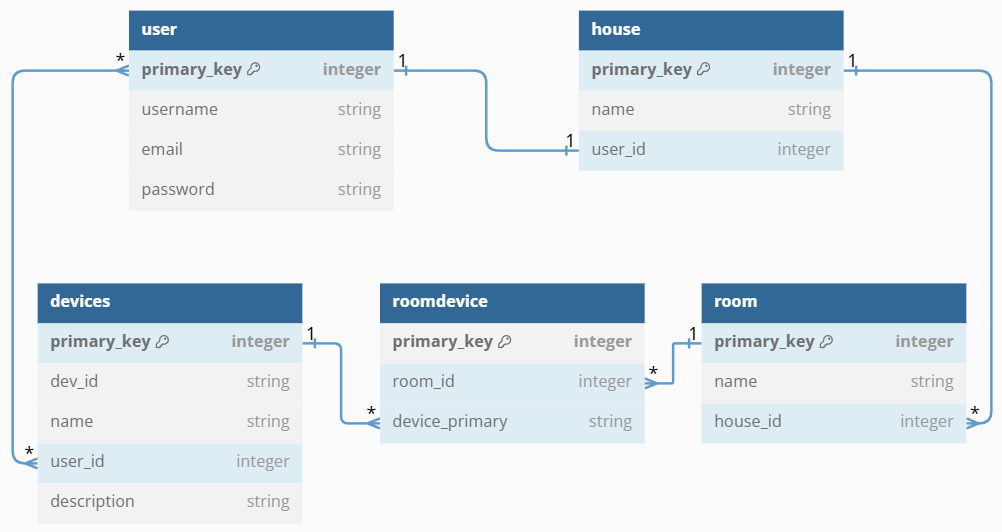
\includegraphics[width=\textwidth]{datenbank.png}
    \caption{Datenbank}
    \label{abb:datenbank}
  \end{figure}
  \begin{itemize}
    \item \textbf{user} --- Enthält die Benutzerdaten.
                        \begin{itemize}
                          \item \textit{\textbf{primary\_key:}} Ein Primärschlüssel vom Typ Integer, der automatisch inkrementiert wird.
                          \item \textit{\textbf{username:}} Der Benutzername, der für jeden Benutzer eindeutig ist.
                          \item \textit{\textbf{email:}} Die E-Mail-Adresse des Benutzers, ebenfalls einzigartig.
                          \item \textit{\textbf{password:}} Das Passwort des Benutzers, das verschlüsselt gespeichert wird.
                        \end{itemize}
                        Ein Benutzer kann mehrere Häuser und Geräte haben.
    \item \textbf{house} --- Speichert die vom Benutzer erstellten Häuser. 
                        \begin{itemize}
                          \item \textit{\textbf{primary\_key:}} Ein Primärschlüssel vom Typ Integer, der automatisch inkrementiert wird.
                          \item \textit{\textbf{name:}} Der vom Benutzer erstellte Name des Hauses.
                          \item \textit{\textbf{user\_id:}} Ein Fremdschlüssel, der auf den Primärschlüssel der Tabelle user verweist, um anzugeben, welchem Benutzer das Haus gehört.
                        \end{itemize}
                        Ein Haus gehört zu einem bestimmten Benutzer. Ein Haus kann mehrere Räume enthalten.
    \item \textbf{room} --- Speichert die vom Benutzer erstellten Räume. 
                        \begin{itemize}
                          \item \textit{\textbf{primary\_key:}} Ein Primärschlüssel vom Typ Integer, der automatisch inkrementiert wird.
                          \item \textit{\textbf{name:}} Der vom Benutzer erstellte Name des Raums.
                          \item \textit{\textbf{house\_id:}} Ein Fremdschlüssel, der auf den Primärschlüssel der Tabelle house verweist.
                        \end{itemize}
                        \par Ein Raum gehört immer zu einem bestimmten Haus. Ein Raum kann mehrere Geräte enthalten.
    \item \textbf{devices} --- Speichert die vom Benutzer angemeldeten Geräte. 
                        \begin{itemize}
                          \item \textit{\textbf{primary\_key:}} Ein Primärschlüssel vom Typ Integer, der automatisch inkrementiert wird.
                          \item \textit{\textbf{dev\_id:}} Die eindeutige, vordefinierte ID des Geräts. 
                          \item \textit{\textbf{name:}} Der vom Benutzer erstellte Name des Geräts.
                          \item \textit{\textbf{user\_id:}} Ein Fremdschlüssel, der auf den Primärschlüssel der Tabelle user verweist und angibt, welchem Benutzer das Gerät gehört.
                          \item \textit{\textbf{description:}} Eine optionale Beschreibung des Geräts.
                        \end{itemize}
                        Ein Gerät gehört genau einem Benutzer und einem Raum. Ein anderes Gerät mit derselben Geräte-ID kann jedoch von einem anderen Benutzer angemeldet und einem anderen Raum zugeordnet werden.
    \item \textbf{roomdevice} --- Speichert die Zuordnung der Geräte zu den Räumen. 
                        \begin{itemize}
                          \item \textit{\textbf{primary\_key:}} Ein Primärschlüssel vom Typ Integer, der automatisch inkrementiert wird.
                          \item \textit{\textbf{room\_id:}} Ein Fremdschlüssel, der auf den Primärschlüssel der Tabelle room verweist.
                          \item \textit{\textbf{device\_primary:}} Ein Fremdschlüssel, der auf den Primärschlüssel der Tabelle device verweist.
                        \end{itemize}
  \end{itemize}
  \paragraph{Aufbau mit SQLAlchemy}
  \par \textbf{}
  \par Jetzt müssen diese Tabellen und deren Verknüpfungen in Form der Modellen in SQLAlchemy definiert werden. Die Models sind in der Datei \texttt{models.py} (Listing \ref{lst:dbmodels}) definiert. 
  \par Zunächst müssen die benötigte Module importiert werden. Das Modul \texttt{bcrypt} wird für die Entschlüssertung und Verifizierung der Passwörter verwendet. Die Module aus der Bibliothek \texttt{sqlalchemy} enthalten die Funktion für die Interaktionen mit der Datenbank. Das Modul \texttt{.base} ist die Datei \texttt{base.py} (Lisitng \ref{lst:dbbase}). Da wird nur ein \texttt{declarative\_base} importiert, und in der Variable \texttt{Base} initialisiert. 
  \begin{lstlisting}[frame=single, style=py, numbers=left, label={lst:dbbase}, caption={db: base.py}]
    from sqlalchemy.orm import declarative_base
    Base = declarative_base()
  \end{lstlisting}  
  \par Die Tabellenmodelle werden in Klassen definiert, die von der \texttt{Base} erben. Dies ist die Standardeinstellung für SQLAlchemy. Die Variable \texttt{\_\_tablename\_\_} legt der Name der Tabelle fest. Die Spalten sind als Objekte der Klasse \texttt{Column} mit gegebenen Parametern definiert. Die Klasse \texttt{UserModel} enthält eine Funktion für die Validierung der Passwörter (Zeile 17). Die Funktion bekommt ein Password-String als Parameter und vergleicht dieser mit dem im Modell gespeicherten Passwort.
  \par In SQLAlchemy, wenn ein \texttt{ChlidModel} Modell einen Fremdschlüssel des \texttt{ParentModel} Modells beinhaltet, muss eine Beziehung mit dem \texttt{ChlidModel} Modell in der \texttt{ParentModel} Klasse definiert werden. Dies wird verwendet, um Datenbankkonflikte beim Löschen oder Aktualisieren von Einträgen im Modell \texttt{ChlidModel} zu vermeiden.
  \par Die Klasse \texttt{HouseModel} enthält neben der Definition der Spalten eine Beziehung zwischen \texttt{HouseModel} und \texttt{RoomModel} im Attribut \texttt{rooms}. Die Beziehung ist so definiert, dass alle zugehörigen Räume gelöscht werden, wenn das Haus gelöscht wird. Außerdem ist in der Klassenvariablen \texttt{\_\_table\_args\_\_} mit dem Befehl \texttt{UniqueConstraint('name', 'user\_id')} (Zeile 27) definiert, dass die Kombination der Spalten \texttt{name} und \texttt{user\_id} eindeutig sein muss. Ein Benutzer kann also nicht 2 Häuser mit dem gleichen Namen anlegen.
  \par Die Klassen \texttt{RoomModel} und \texttt{DeviceModel} haben eine Beziehung zur Klasse \texttt{RoomDeviceModel}, und in der Klasse \texttt{RoomDeviceModel} werden die Beziehungen zu den beiden Klassen definiert. Damit wird sichergestellt, dass beim Löschen eines Raumes oder eines Gerätes auch die entsprechende Verknüpfung gelöscht wird. Dabei ist zu beachten, dass beim Löschen eines Raumes das zum Raum gehörende Gerät nicht gelöscht wird und umgekehrt.
  \paragraph{Interaktionen mit der Datenbank}
  \textbf{}
  \par In der Datei \texttt{queries.py} (Listing \ref{lst:dbqueries}) sind die benötigten Funktionen für die Interaktion mit der Datenbank definiert. Diese Funktionen ermöglichen das Einfügen, Löschen, Abrufen und Aktualisieren der Daten in der Datenbank.
  \par Jede Funktion bekommt ein \texttt{AsyncSession} als erster Parameter. Über diese Session werden die Operationen in der Datenbank duchgeführt. Das erlaubt auch asynchroner Zugriff zur Datenbank. Das Erzeugen der Sessions wird im nächsten Paragraph beschrieben. 
  \par Als Beispiel werde ich die Struktur der Funktion \texttt{add\_user()} näher erläutern. Diese Funktion fügt einen neuen Benutzer in die Datenbank ein. Die Funktion erhält als Parameter \texttt{AsyncSession} und die Benutzerdaten, d.h. Benutzername, Email und Passwort. Zuerst wird das Passwort verschlüsselt. Anschließend wird ein Objekt \texttt{new\_user} der Klasse \texttt{UserModel} mit den übergebenen Parametern erzeugt. Dieses Objekt wird mit dem Befehl \texttt{db\_session.add(new\_user)} in die Datenbank eingefügt. Nach dem Einfügen muss der Befehl \texttt{db\_session.commit()} aufgerufen werden, um die Änderungen in der Datenbank zu speichern. Anschließend wird das \texttt{new\_user} aktualisiert und der Primärschlüssel zurückgegeben.
  \par Beim Arbeiten mit der Datenbank müssen mögliche Fehler behandelt werden. Deshalb enthält jede Funktion einen \texttt{Try-Catch-Block}. 
  \par Ein \texttt{IntegrityError} wird ausgelöst, wenn eine Datenbankoperation gegen eine Integritätsbedingung der Datenbank verletzt. Er wird bei Verletzung einer Fremdschlüsselbeziehung, der Unique Constraints oder beim Einfügen von Daten des falschen Typs erzeugt. 
  \par Ein \texttt{SQLAlchemyError} umfasst alle Fehler, die von SQLAlchemy ausgelöst werden, wenn die Operation nicht erfolgreich war. Dieser Fehler wird bei Syntaxfehlern in der SQL-Abfrage oder bei Fehlern in der Datenbankverbindung ausgelöst.
  \par Alle anderen möglichen Fehler, die keine \texttt{SQLAlchemy}-Fehler sind, werden im Block \texttt{Exception} gesammelt.
  \par Bei jedem Fehler wird der Fehler geloggt und die Session zurückgesetzt, damit keine unvollständigen Daten in der Datenbank gespeichert werden. Anschließend wird eine \texttt{HTTPException} mit Status und Beschreibung des Fehlers zurückgegeben.
  \paragraph{Initialisierung der Datenbank}
  \par \textbf{}
  \par Beim Import des Moduls \texttt{db} wird die Klasse \texttt{\_\_init\_\_} (Listing \ref{lst:dbinit}) aufgerufen. In dieser Klasse wird zunächst der Logger initialisiert. Anschließend wird eine asynchrone Engine \texttt{async\_engine} für die Verbindung zur Datenbank erzeugt. Mit dem Parameter \texttt{async\_engine} wird das Objekt \texttt{async\_session} der Klasse \texttt{Sessionmaker} erzeugt. Die Funktion \texttt{create\_tables()} initialisiert alle Tabellen in den Klassenmodellen, die von der Klasse \texttt{Base} erben. Die Funktion \texttt{get\_session()} gibt eine asynchrone Session aus der \texttt{async\_session} zurück. Mit dieser Session wird dann auf die Datenbank zugegriffen.
  \subsubsection{Webserver} 
  \subsubsection{Frontend}
  \subsubsection{Integration der Komponenten}
  \par MQtt client, erhalten Daten von Broker etc

\newpage
\section{Ergebnisse und Diskussion}

\newpage
\section{Quellen}
\begin{thebibliography}{20}
  \bibitem{pa1}
  O. Baida,
  \textit{Anbindung der Sensoren und Aktoren an den Arduino zur Realisierung eines Sicherheitssystems},
  Projektarbeit 1, 2024.

  \bibitem{pa2}
  O. Baida, Projektarbeit 2 \textit{Sicherheitssystem fur das Haus basierend auf Arduino, ESP8266 \& Raspberry Pi} \url{https://github.com/oleksiibaida/PA2.git}
  \bibitem{video}
  
  \bibitem{statita_smhomes}
  Statista, \textit{„Smart Home - Anzahl der Haushalte in Deutschland 2028“}, Zugegriffen: 13. Januar 2025. [Online]. Verfügbar unter \url{https://de.statista.com/prognosen/885611/anzahl-der-smart-home-haushalte-in-deutschland}
  \bibitem{spiegel_heizung}
  J. Breithut, \textit{„Strom und Heizung: Wann ein Smart Home wirklich beim Energiesparen hilft“}, Der Spiegel, 17. Juli 2022. Zugegriffen: 13. Januar 2025. [Online]. Verfügbar unter: \url{https://www.spiegel.de/netzwelt/gadgets/strom-und-heizung-wann-ein-smart-home-wirklich-beim-energiesparen-hilft-a-ffb4b710-0cec-40e4-a2c4-6c5d4a3feb92}


  \par \textbf{Links zur verwendeten Hardware:}
  \bibitem{arduino}
  Arduino.cc, \textit{Arduino UNO}, \url{https://docs.arduino.cc/hardware/uno-rev3/}
  \bibitem{raspi}
  Raspberry Pi Foundation, \textit{Raspberry Pi 1 B+}, \url{https://www.raspberrypi.com/products/raspberry-pi-1-model-b-plus/}
  \bibitem{esp8266}
  Espressif, \textit{ESP8266}, \url{https://www.espressif.com/}, \url{https://www.electronicwings.com/sensors-modules/esp8266-wifi-module}
  \par \textbf{Links zur verwendeten Software:}
  \bibitem{mqtt}
  Dr Andy Stanford-Clark, Arlen Nipper, \textit{Message Queuing Telemetry Transport}, \url{https://mqtt.org/}
  \bibitem{python}
  Guido van Rossum, Python Software Foundation, \textit{Python}, \url{https://www.python.org/}
  \bibitem{telegram}
  Telegram FZ-LLC, \textit{Telegram Messenger}, \url{https://github.com//telegramdesktop/tdesktop}
  \par \textbf{Linux-Packete}:
  \bibitem{hostapd}
  Jouni Malinen, \textit{hostapd}, \url{https://w1.fi/hostapd/}, Zugriff am: 19. September 2024.
  \bibitem{dnsmasq}
  Simon Kelley, \textit{dnsmasq}, \url{https://dnsmasq.org/doc.html}, Zugriff am: 20. September 2024.
  \bibitem{mosquitto}
  Eclipse Foundation, \textit{Eclipse Mosquitto}, \url{https://mosquitto.org/}
  \par \textbf{ESP- und Arduino-Bibliotheken}
  \bibitem{pubsub} 
  Knolleary, \textit{PubSubClient}, \url{https://pubsubclient.knolleary.net/}, Zugriff am: 21. Oktober 2024.
  \bibitem{espwifi}
  ESPWIFI.h, \url{https://arduino-esp8266.readthedocs.io/en/latest/esp8266wifi/readme.html}
  \bibitem{eeprom}
  EEPROM.h, \url{https://docs.arduino.cc/learn/built-in-libraries/eeprom/}
  \bibitem{keypad}
  Keypad.h \url{https://docs.arduino.cc/libraries/keypad/}
  \bibitem{scholz}
  R. Scholz, \textit{Syncloop}, Persönliche Mitteilungen
  \par \textbf{Python-Bibliotheken}
  \bibitem{paho}
  Pierre Fersing, Roger Light \textit{paho-mqtt}, \url{https://pypi.org/project/paho-mqtt/}, Zugriff am: 21. Oktober 2024.
  \bibitem{tgbot}
  Open Source, \textit{python-telegram-bot}, \url{https://docs.python-telegram-bot.org/en/v21.6/}
  \bibitem{json}
  Python Software Foundation, \textit{json}, \url{https://docs.python.org/3/library/json.html}
  \bibitem{threading}
  Python Software Foundation, \textit{threading}, \url{https://docs.python.org/3/library/threading.html}
  \bibitem{queue}
  Python Software Foundation, \textit{queue}, \url{https://docs.python.org/3/library/queue.html}
  \bibitem{sqlite}
  Gerhard Häring, \textit{sqlite3}, \url{https://docs.python.org/3/library/sqlite3.html}
  \bibitem{pyzbar}
  Lawrence Hudson, \textit{pyzbar}, \url{https://github.com/NaturalHistoryMuseum/pyzbar/}
  \bibitem{cv2}
  Intel, \textit{OpenCV}, \url{https://github.com/opencv/opencv-python}
  \bibitem{aiohttp}
  Aio-Libs, \textit{aiohttp}, \url{https://github.com/aio-libs/aiohttp}
\end{thebibliography}



\listoffigures
\addcontentsline{toc}{section}{Abbildungsverzeichnis}

\listoftables
%\addcontentsline{toc}{section}{Tabellenverzeichnis}
% \lstlistoflistings
% \addcontentsline{toc}{section}{Programmcode}
\newpage
\section{Programmcode}

\begin{lstlisting}[frame=single, style=cpp, numbers=left, label={lst:esp8266setup}, caption={ESP: setup}]
  void setup()
  {
    Serial.begin(9600);
    // GET WiFi Daten aus EEPROM
    EEPROM.begin(128);
    char eeprom_ssid[MAX_SSID_LENGTH] = {0};
    char eeprom_password[MAX_PASSWORD_LENGTH] = {0};
    EEPROM.get(0, eeprom_ssid);
    EEPROM.get(32, eeprom_password);
    EEPROM.end();
    // Daten gefunden
    if (is_valid_string(eeprom_ssid, MAX_SSID_LENGTH) && is_valid_string(eeprom_password, MAX_PASSWORD_LENGTH))
    {
      if (connect_wifi(eeprom_ssid, eeprom_password))
      {
        connect_mqtt();
        return;
      }
    }
    // keine WLAN-DAten gefunden
    setup_ap();
  }
\end{lstlisting}
\begin{lstlisting}[frame=single, style=cpp, numbers=left, label={lst:esp8266validstring}, caption={ESP: is\_valid\_string}]
  bool is_valid_string(char *data, int max_length)
  {
    if (strlen(data) == 0 or strlen(data) > max_length)
      return false;
    for (int i = 0; i < max_length; i++)
    {
      if (data[i] == '\0')
        return true; // End of valid String
      if (data[i] == 0xFF) // Default EEPROM
        return false;
    }
    return false;
  }
\end{lstlisting}
\begin{lstlisting}[frame=single, style=cpp, numbers=left, label={lst:espconnectwifi}, caption={ESP: connect\_wifi}]
  bool connect_wifi(char *ssid, char *password)
  {
    WiFi.mode(WIFI_STA);
    WiFi.begin(ssid, password);
  
    for (uint8_t i = 0; i < wifi_repeat; i++)
    {
      if (WiFi.status() == WL_CONNECTED)
      {
        Serial.println(WiFi.localIP());
        return true;
      }
      delay(1000);
    }
    return false;
  }
\end{lstlisting}
\begin{lstlisting}[frame=single, style=cpp, numbers=left, label={lst:espconnectmqtt}, caption={ESP: connect\_mqtt}]
  void mqtt_connect()
  {
    set_topics();
    mqttClient.setServer(MQTT_BROKER_ADRRESS, MQTT_PORT);
    mqttClient.setCallback(callback);
    for (int i = 0; i < wifi_repeat; i++)
    {
      if (mqttClient.connect(DEVICE_ID))
        mqttClient.subscribe(SUBSCRIBE_TOPIC);
        return;
      else
        delay(1000);
    }
  }
\end{lstlisting}
\begin{lstlisting}[frame=single, style=cpp, numbers=left, label={lst:espsettopics}, caption={ESP: set\_topics}]
  void set_topics()
  {
    SUBSCRIBE_TOPIC = (char *)malloc(strlen(TOPIC_COMMAND) + strlen(DEVICE_ID) + 2);
    PUBLISH_TOPIC = (char *)malloc(strlen("data") + strlen(DEVICE_ID) + 2);
  
    strcpy(SUBSCRIBE_TOPIC, TOPIC_COMMAND);
    strcat(SUBSCRIBE_TOPIC, "/");
    strcat(SUBSCRIBE_TOPIC, DEVICE_ID);
  
    strcpy(PUBLISH_TOPIC, "data");
    strcat(PUBLISH_TOPIC, "/");
    strcat(PUBLISH_TOPIC, DEVICE_ID);
  }
\end{lstlisting}
\begin{lstlisting}[frame=single, style=cpp, numbers=left, label={lst:esp8266defap}, caption={ESP8266: ap\_konfiguration}]
  const char AP_SSID[] = "ESP8266";
  const char AP_PASSWORD[] = "setupesp";
  IPAddress ap_ip(10, 0, 0, 1);
  IPAddress ap_gateway(10, 0, 0, 1);
  IPAddress ap_subnet(255, 255, 255, 0);
  AsyncWebServer server(80);
  const String html_page = R"rawliteral(
    <html>
    <body>
      <h2>Wi-Fi Configuration</h2>
      <form action="/save" method="POST">
        SSID:<br>
        <input type="text" name="ssid" required><br>
        Password:<br>
        <input type="password" name="password" required><br><br>
        <input type="submit" value="Submit">
      </form>
    </body>
    </html>
  )rawliteral";
\end{lstlisting}
\begin{lstlisting}[frame=single, style=cpp, numbers=left, label={lst:esp8266setupap}, caption={ESP: setup\_ap}]
  void setup_ap()
  {
    WiFi.mode(WIFI_AP);
    WiFi.softAP(AP_SSID, AP_PASSWORD);
    WiFi.softAPConfig(ap_ip, ap_gateway, ap_subnet);
  
    server.on("/", HTTP_GET, [](AsyncWebServerRequest *request)
              { request->send(200, "text/html", html_page); });
  
    server.on("/save", HTTP_POST, [](AsyncWebServerRequest *request)
              {
                // get input data
                String ssid = request->getParam("ssid", true)->value();
                String password = request->getParam("password", true)->value();
                if (ssid.length() > MAX_SSID_LENGTH - 1 || password.length() > MAX_PASSWORD_LENGTH - 1)
                {
                  return;
                }
                // String in char[]
                char new_ssid[MAX_SSID_LENGTH] = {0};
                strncpy(new_ssid, ssid.c_str(), MAX_SSID_LENGTH - 1);
                char new_password[MAX_PASSWORD_LENGTH] = {0};
                strncpy(new_password, password.c_str(), MAX_PASSWORD_LENGTH - 1);
  
                // in EEPROM speichern
                EEPROM.begin(128);
                EEPROM.put(0, new_ssid);
                EEPROM.put(32, new_password);
                EEPROM.commit();
                EEPROM.end();
  
                request->send(200, "text/html", "WiFi saved. Rebooting...");
                ESP.restart(); });
  
    server.begin();
  }
\end{lstlisting}

\begin{lstlisting}[frame=single, style=cpp, numbers=left, label={lst:esp8266readserial}, caption={ESP8266: readSerialData}]
  void readSerialData()
  {
    if (Serial.available() > 0)
    {
      String readString = "";
      // Lese Daten aus Serial als String ab
      readString = Serial.readStringUntil('\n');
      if (sizeof(readString) > buss_serial)
        return;
      // String in char-Feld konvertieren
      char readSerialChar[readString.length() + 1];
      readString.toCharArray(readSerialChar, readString.length() + 1);    
      // Suche Position von ':'
      char *delim_pos = strchr(readSerialChar, ':');
      if (delim_pos != NULL)
      {
        size_t topic_length = delim_pos - readSerialChar;
        char topic[topic_length + 1];
        strncpy(topic, readSerialChar, topic_length);
        topic[topic_length] = '\0';
        char *message = delim_pos + 1;
        PUBLISH_TOPIC = (char *)malloc(strlen(CLIENT_ID) + strlen(topic) + 2);
        if (PUBLISH_TOPIC == NULL)
        {
          PUBLISH_TOPIC = topic;
        }
        else
        {
          strcpy(PUBLISH_TOPIC, topic);
          strcat(PUBLISH_TOPIC, "/");
          strcat(PUBLISH_TOPIC, CLIENT_ID);
        }
        // MQTT-Nachricht senden
        mqttClient.publish(PUBLISH_TOPIC, message);
      }
      else // kein : gefunden
        return;
    }
  }
\end{lstlisting}

\begin{lstlisting}[frame=single, style=cpp, numbers=left, label={lst:esp8266callback}, caption={ESP8266: callback}]
  void callback(char *topic, byte *payload, unsigned int length)
  {
    String id = String(topic).substring(String(topic).indexOf('/') + 1);
    if (id == CLIENT_ID)
    {
      String text = "";
      for (int i = 0; i < length; i++)
      {
        text += (char)payload[i];
      }
      text.trim();
      // Print in Arduino
      Serial.println(text);
    }
  }
\end{lstlisting}

\begin{lstlisting}[frame=single, style=py, numbers=left, label={lst:dbmodels}, caption={db: models.py}]
  import bcrypt
  from sqlalchemy import Column, Integer, String, ForeignKey, PrimaryKeyConstraint
  from sqlalchemy.orm import relationship
  from sqlalchemy.schema import UniqueConstraint
  from .base import Base
  from app.config import Config
  __logger = Config.logger_init()
  
  
  class UserModel(Base):
      __tablename__ = 'user'
      primary_key = Column(Integer, primary_key=True, autoincrement=True, nullable=False)
      username = Column(String(50), unique=True, nullable=False)
      email = Column(String(100), unique=True, nullable=False)
      password = Column(String(200), nullable=False)
      
      def verify_password(self, password:str):
          return bcrypt.checkpw(password.encode('utf-8'), self.password)
  
  class HouseModel(Base):
      __tablename__ = 'house'
      primary_key = Column(Integer, primary_key=True, autoincrement=True, nullable=False)
      name = Column(String(50), nullable=False)
      user_id = Column(Integer, ForeignKey("user.primary_key", ondelete='CASCADE'), nullable=False)
      rooms = relationship("RoomModel", backref="house", cascade="all, delete-orphan", lazy='selectin')
  
      __table_args__ = (UniqueConstraint('name', 'user_id'),)
  
  class RoomModel(Base):
      __tablename__ = 'room'
      primary_key = Column(Integer, primary_key=True, autoincrement=True, nullable=False)
      name = Column(String(50), nullable=False)
      house_id = Column(Integer, ForeignKey('house.primary_key', ondelete='CASCADE'), nullable=False)
      
      devices = relationship("RoomDeviceModel", back_populates="room", cascade="all, delete-orphan", lazy='selectin')
  
      __table_args__ = (UniqueConstraint('name', 'house_id'),)
  
  class DeviceModel(Base):
      __tablename__ = 'device'
      primary_key = Column(Integer, primary_key=True, autoincrement=True, nullable=False)
      dev_id = Column(String(10), nullable=False)
      name = Column(String(50), nullable=False)
      user_id = Column(Integer, ForeignKey('user.primary_key', ondelete='CASCADE'), nullable=False, unique=False)
      description = Column(String(250), nullable=True)
      dev_rooms = relationship("RoomDeviceModel", back_populates="device", cascade="all, delete-orphan", lazy='selectin')
  
      __table_args__ = (UniqueConstraint('user_id', 'dev_id'),)
  
  class RoomDeviceModel(Base):
      __tablename__ = 'room_device'
      primary_key = Column(Integer, primary_key=True, autoincrement=True, nullable=False)
      room_id = Column(Integer, ForeignKey('room.primary_key', ondelete='CASCADE'), nullable=False)
      device_primary = Column(Integer, ForeignKey('device.primary_key', ondelete='CASCADE'), nullable=False)
  
      room = relationship("RoomModel", back_populates="devices")
      device = relationship("DeviceModel", back_populates="dev_rooms")
  
      __table_args__ = (UniqueConstraint('room_id', 'device_primary'),)
    \end{lstlisting}
\begin{lstlisting}[frame=single, style=py, numbers=left, label={lst:dbqueries}, caption={db: queries.py}]
  import bcrypt
  from app.config import Config
  from sqlalchemy import select, insert, update, delete, func
  from sqlalchemy.exc import IntegrityError, NoResultFound, SQLAlchemyError
  from sqlalchemy.ext.asyncio import AsyncSession
  from sqlalchemy.orm import joinedload
  from .models import UserModel, HouseModel, RoomModel, DeviceModel, RoomDeviceModel
  from fastapi import Depends, HTTPException
  _logger = Config.logger_init()
  
  async def add_user(db_session: AsyncSession, username: str, email: str, password: str):
      """
      Adds new user to Database. SIGNUP.
      :param db_session: SQLAlchemy AsyncSession
      :param username, email, password: user data
      :return: True -> user added; IntegityError -> username or email already in DB; HTTPExcepion
      """
      if username is None or email is None or password is None:
          _logger.error("All user data must be provided")
          return False
      try:
          password = bcrypt.hashpw(password.encode('utf-8'), bcrypt.gensalt())
          new_user = UserModel(username=username, email=email, password=password)
          _logger.debug(f'ADD U_NAME {new_user.username} START')
          db_session.add(new_user)
          await db_session.commit()
          await db_session.refresh(new_user)
          _logger.debug(f'ADD U_NAME {new_user.username} COMPLETED')
          return new_user.primary_key
      except IntegrityError as e:
          _logger.error(f"IntegrityError: {e}")
          await db_session.rollback()
          raise HTTPException(status_code=422, detail="ALREADY EXISTS")
      except SQLAlchemyError as e:
          _logger.error(f"SQLAlchemyError: {e}")
          await db_session.rollback()
          raise HTTPException(status_code=500, detail="DATABASE ERROR")
      except Exception as e:
          _logger.error(f"Exception: {e}")
          await db_session.rollback()
          raise HTTPException(status_code=500, detail="UNEXPECTED DATABASE ERROR")
  
  async def get_user_data(db_session: AsyncSession, user_primary: int = None, username: str = None, email: str = None):
      if not user_primary and not username and not email:
          _logger.error(msg="EMPTY SET")
          raise ValueError()
      query = select(UserModel)
      if user_primary:
          query = query.where(UserModel.primary_key == user_primary)
      if username:
          query = query.where(UserModel.username == username)
      if email:
          query = query.where(UserModel.email == email)
      try:
          res = await db_session.execute(query)
          return res.scalars().first()
      except IntegrityError as e:
          _logger.error(f"IntegrityError: {e}")
          await db_session.rollback()
          raise HTTPException(status_code=422, detail="NOT FOUND")
      except SQLAlchemyError as e:
          _logger.error(f"SQLAlchemyError: {e}")
          await db_session.rollback()
          raise HTTPException(status_code=500, detail="DATABASE ERROR")
      except Exception as e:
          _logger.error(f"Exception: {e}")
          await db_session.rollback()
          raise HTTPException(status_code=500, detail="UNEXPECTED DATABASE ERROR")
  
  async def add_new_house(db_session: AsyncSession, user_primary: int, house_name: str):
      try:
          new_house = HouseModel(user_id=user_primary, name=house_name)
          db_session.add(new_house)
          await db_session.commit()
          await db_session.refresh(new_house)
          _logger.info(f"U_ID: {user_primary} ADD HOUSE_ID {new_house.primary_key}")
          return new_house
      except IntegrityError as e:
          _logger.error(f"IntegrityError: {e}")
          await db_session.rollback()
          raise HTTPException(status_code=422, detail="ALREADY EXISTS")
      except SQLAlchemyError as e:
          _logger.error(f"SQLAlchemyError: {e}")
          await db_session.rollback()
          raise HTTPException(status_code=500, detail="DATABASE ERROR")
      except Exception as e:
          _logger.error(f"Exception: {e}")
          await db_session.rollback()
          raise HTTPException(status_code=500, detail="UNEXPECTED DATABASE ERROR")
  
  async def delete_house(db_session: AsyncSession, house_id):
      try:
          house = await db_session.get(HouseModel, house_id)
          await db_session.delete(house)
          await db_session.commit()
          return True
      except IntegrityError as e:
          _logger.error(f"IntegrityError: {e}")
          await db_session.rollback()
          raise HTTPException(status_code=422, detail="NOT FOUND")
      except SQLAlchemyError as e:
          _logger.error(f"SQLAlchemyError: {e}")
          await db_session.rollback()
          raise HTTPException(status_code=500, detail="DATABASE ERROR")
      except Exception as e:
          _logger.error(f"Exception: {e}")
          await db_session.rollback()
          raise HTTPException(status_code=500, detail="UNEXPECTED DATABASE ERROR")
  
  async def get_house(db_session: AsyncSession, house_primary: int):
      try:
          return await db_session.get(HouseModel, house_primary)
      except NoResultFound:
          _logger.error(f'HOUSE_ID {house_primary} HOUSE NOT FOUND')
          raise HTTPException(status_code=404, detail='NOT FOUND')
      except IntegrityError as e:
          _logger.error(f"IntegrityError: {e}")
          await db_session.rollback()
          raise HTTPException(status_code=422, detail="NOT FOUND")
      except SQLAlchemyError as e:
          _logger.error(f"SQLAlchemyError: {e}")
          await db_session.rollback()
          raise HTTPException(status_code=500, detail="DATABASE ERROR")
      except Exception as e:
          _logger.error(f"Exception: {e}")
          await db_session.rollback()
          raise HTTPException(status_code=500, detail="UNEXPECTED DATABASE ERROR")
  
  async def get_houses_on_user(db_session: AsyncSession, user_primary: int):
      try:
          stmt = (
              select(HouseModel)
              .options(
                  joinedload(HouseModel.rooms)
                  .joinedload(RoomModel.devices)
                  .joinedload(RoomDeviceModel.device)
                  .joinedload(DeviceModel.dev_rooms)
              )
              .filter(HouseModel.user_id == user_primary)
          )
          # print(str(stmt))
          houses = await db_session.execute(stmt)
          houses = houses.scalars().unique().all()
          return houses
      except NoResultFound:
          _logger.error(f'U_ID {user_primary} HOUSE NOT FOUND')
          raise HTTPException(status_code=404, detail='NOT FOUND')
      except IntegrityError as e:
          _logger.error(f"IntegrityError: {e}")
          await db_session.rollback()
          raise HTTPException(status_code=422, detail="NOT FOUND")
      except SQLAlchemyError as e:
          _logger.error(f"SQLAlchemyError: {e}")
          await db_session.rollback()
          raise HTTPException(status_code=500, detail="DATABASE ERROR")
      except Exception as e:
          _logger.error(f"Exception: {e}")
          await db_session.rollback()
          raise HTTPException(status_code=500, detail="UNEXPECTED DATABASE ERROR")
      
  async def get_house_by_room(db_session: AsyncSession, room_id: int):
      try:
          stmt = select(HouseModel).join(RoomModel, RoomModel.house_id == HouseModel.primary_key).where(RoomModel.primary_key == room_id)
          res = await db_session.execute(stmt)
          return res.scalar_one_or_none()
      except NoResultFound as e:
          _logger.error(f"NoResultFound:{e}")
          raise HTTPException(404, 'NOT FOUND')
      except IntegrityError as e:
          _logger.error(f"IntegrityError: {e}")
          await db_session.rollback()
          raise HTTPException(status_code=422, detail="NOT FOUND")
      except SQLAlchemyError as e:
          _logger.error(f"SQLAlchemyError: {e}")
          await db_session.rollback()
          raise HTTPException(status_code=500, detail="DATABASE ERROR")
      except Exception as e:
          _logger.error(f"Exception: {e}")
          await db_session.rollback()
          raise HTTPException(status_code=500, detail="UNEXPECTED DATABASE ERROR")
      
  async def verify_house_owner(db_session: AsyncSession, user_primary: int, house_id: int):
      try:
          house = await db_session.get(HouseModel, house_id)
          if house:
              return house.user_id == user_primary
      except NoResultFound as e:
          _logger.error(f"NoResultFound: {e}")
          raise HTTPException(404, 'NOT FOUND')
      except IntegrityError as e:
          _logger.error(f"IntegrityError: {e}")
          await db_session.rollback()
          raise HTTPException(status_code=422, detail="NOT FOUND")
      except SQLAlchemyError as e:
          _logger.error(f"SQLAlchemyError: {e}")
          await db_session.rollback()
          raise HTTPException(status_code=500, detail="DATABASE ERROR")
      except Exception as e:
          _logger.error(f"Exception: {e}")
          await db_session.rollback()
          raise HTTPException(status_code=500, detail="UNEXPECTED DATABASE ERROR")
  
  async def add_new_room(db_session: AsyncSession, house_id: int, room_name: str):
      try:
          new_room = RoomModel(name = room_name, house_id = house_id)
          db_session.add(new_room)
          await db_session.commit()
          _logger.info(f"ADD ROOM_NAME {room_name} HOUSE_ID {house_id}")
          return True
      except NoResultFound as e:
          _logger.error(f"NoResultFound:{e}")
          raise HTTPException(404, 'NOT FOUND')
      except IntegrityError as e:
          _logger.error(f"IntegrityError: {e}")
          await db_session.rollback()
          raise HTTPException(status_code=422, detail="ALREADY EXISTS")
      except SQLAlchemyError as e:
          _logger.error(f"SQLAlchemyError: {e}")
          await db_session.rollback()
          raise HTTPException(status_code=500, detail="DATABASE ERROR")
      except Exception as e:
          _logger.error(f"Exception: {e}")
          await db_session.rollback()
          raise HTTPException(status_code=500, detail="UNEXPECTED DATABASE ERROR")
  
  async def delete_room(db_session: AsyncSession, room_id: int):
      try:
          # get RoomModel from DB
          del_room = await db_session.execute(
              select(RoomModel)
              .where(RoomModel.primary_key == room_id)
          )
          # fetch result
          del_room = del_room.scalars().one()
  
          await db_session.delete(del_room)
          await db_session.commit()
          return True
      except NoResultFound as e:
          _logger.error(f"NoResultFound:{e}")
          raise HTTPException(404, 'NOT FOUND')
      except IntegrityError as e:
          _logger.error(f"IntegrityError: {e}")
          await db_session.rollback()
          raise HTTPException(status_code=422, detail="NOT FOUND")
      except SQLAlchemyError as e:
          _logger.error(f"SQLAlchemyError: {e}")
          await db_session.rollback()
          raise HTTPException(status_code=500, detail="DATABASE ERROR")
      except Exception as e:
          _logger.error(f"An unexpected error: {e}")
          await db_session.rollback()
          raise HTTPException(status_code=500, detail="UNEXPECTED DATABASE ERROR")
      
  async def add_new_device(db_session: AsyncSession, user_id: int, device_data):
      try:
          if device_data.dev_id is None or device_data.name is None or user_id is None:
              return False
          new_dev = DeviceModel(
              dev_id = device_data.dev_id,
              name = device_data.name,
              user_id = user_id,
              description = device_data.description
          )
          db_session.add(new_dev)
          await db_session.commit()
          await db_session.refresh(new_dev)
          return new_dev
      except NoResultFound as e:
          _logger.error(f"NoResultFound:{e}")
          raise HTTPException(404, 'NOT FOUND')
      except IntegrityError as e:
          await db_session.rollback()
          _logger.error(f"IntegrityError: {e}")
          raise HTTPException(status_code=422, detail="ALREADY EXISTS")
      except SQLAlchemyError as e:
          await db_session.rollback()
          _logger.error(f"SQLAlchemyError: {e}")
          raise HTTPException(status_code=500, detail="DATABASE ERROR")
      except Exception as e:
          await db_session.rollback()
          _logger.error(f"An unexpected error: {e}")
          raise HTTPException(status_code=500, detail="DATABASE ERROR")
      
  async def get_device(db_session:AsyncSession, user_id: int, primary_key: int = None, dev_id: str = None, name: str = None):
      """
      Get Device data
      :param db_session: AsyncSession to access DB
      :param user_id: Owner of the Sensor
      :param id: Optional; device.primary_key in DB
      :param dev_id: Optional; device.dev_id (Factory ID)
      :param name: OPtional Device Name
      """
      
      if not primary_key and not dev_id and not name:
          return None
      stmt = select(DeviceModel)
      if primary_key:
          stmt = stmt.where(DeviceModel.primary_key == primary_key, DeviceModel.user_id == user_id)
      if dev_id:
          stmt = stmt.where(DeviceModel.dev_id == dev_id, DeviceModel.user_id == user_id)
      if name:
          stmt = stmt.where(DeviceModel.name == name, DeviceModel.user_id == user_id)
      try:
          res = await db_session.execute(stmt)
          return res.scalar_one_or_none()
      except NoResultFound:
          return None
      except IntegrityError as e:
          await db_session.rollback()
          _logger.error(f"IntegrityError: {e.orig}")
          raise HTTPException(status_code=422, detail="NOT FOUND")
      except SQLAlchemyError as e:
          await db_session.rollback()
          _logger.error(f"SQLAlchemyError: {e}")
          raise HTTPException(status_code=500, detail="DATABASE ERROR")
      except Exception as e:
          await db_session.rollback()
          _logger.error(f"An unexpected error: {e}")
          raise HTTPException(status_code=500, detail="UNEXPECTED DATABASE ERROR")
      
  async def get_devices_on_user(db_session: AsyncSession, user_primary: int):
      try:
          stmt = (
              select(DeviceModel)
              .options(
                  joinedload(DeviceModel.dev_rooms)
                  .joinedload(RoomDeviceModel.room)
                  .joinedload(RoomModel.devices)
              )
              .filter(DeviceModel.user_id == user_primary)
          )        
          
          devices = await db_session.execute(stmt)
          return devices.scalars().unique().all()
      except NoResultFound:
          _logger.error(f'U_ID {user_primary} HOUSE NOT FOUND')
          raise HTTPException(status_code=404, detail='NOT FOUND')
      except IntegrityError as e:
          _logger.error(f"IntegrityError: {e}")
          await db_session.rollback()
          raise HTTPException(status_code=422, detail="NOT FOUND")
      except SQLAlchemyError as e:
          _logger.error(f"SQLAlchemyError: {e}")
          await db_session.rollback()
          raise HTTPException(status_code=500, detail="DATABASE ERROR")
      except Exception as e:
          _logger.error(f"Exception: {e}")
          await db_session.rollback()
          raise HTTPException(status_code=500, detail="UNEXPECTED DATABASE ERROR")
      
  async def update_device(db_session: AsyncSession, user_id:int, new_device_data):
      try:
          # TODO also change room
          if new_device_data.primary is None:
              _logger.error("DEVICE_PRIMARY IS NOT PROVIDED")
              raise HTTPException(status_code=400, detail="DEVICE_PRIMARY IS NOT PROVIDED")
          if new_device_data.name is None and new_device_data.description is None:
              _logger.error("NEW DATA IS NOT PROVIDED")
              raise HTTPException(status_code=400, detail="NEW DATA IS NOT PROVIDED")
          device = await db_session.get(DeviceModel, new_device_data.primary)
          if device:
              if device.user_id != user_id:
                  _logger.critical(f"UNAUTHORIZED ACCESS U_ID {user_id} ON DEVICE {device.primary_key}")
                  raise HTTPException(status_code=401, detail="User is not owner of this device")
              if new_device_data.name:
                  device.name = new_device_data.name
              if new_device_data.description:
                  device.description = new_device_data.description
              await db_session.commit()
          return device
      except NoResultFound:
          _logger.error(f'{new_device_data.primary} DEVICE NOT FOUND')
          raise HTTPException(status_code=404, detail='NOT FOUND')
      except IntegrityError as e:
          _logger.error(f"IntegrityError: {e}")
          await db_session.rollback()
          raise HTTPException(status_code=422, detail="NOT FOUND")
      except SQLAlchemyError as e:
          _logger.error(f"SQLAlchemyError: {e}")
          await db_session.rollback()
          raise HTTPException(status_code=500, detail="DATABASE ERROR")
      except HTTPException as e:
          raise e
      except Exception as e:
          _logger.error(f"Exception: {e}")
          await db_session.rollback()
          raise HTTPException(status_code=500, detail="UNEXPECTED DATABASE ERROR")
      
  async def delete_device(db_session: AsyncSession, device_primary_key: int, device_id: str = None):
      try:
          if not device_id and not device_primary_key:
              _logger.error("EMPTY SET")
              raise HTTPException(status_code=400, detail="NO DEVICE DATA PROVIDED")
          # del_device = DeviceModel(primary_key = device_primary_key, dev_id = device_id)
          del_device = await db_session.get(DeviceModel, device_primary_key)
          if del_device:
              await db_session.delete(del_device)
              await db_session.commit()
              return True
          else:
              raise HTTPException(404, 'NOT FOUND')
      except NoResultFound as e:
          _logger.error(f"NoResultFound:{e}")
          raise HTTPException(404, 'NOT FOUND')
      except IntegrityError as e:
          _logger.error(f"IntegrityError: {e}")
          await db_session.rollback()
          raise HTTPException(status_code=422, detail="NOT FOUND")
      except SQLAlchemyError as e:
          _logger.error(f"SQLAlchemyError: {e}")
          await db_session.rollback()
          raise HTTPException(status_code=500, detail="DATABASE ERROR")
      except Exception as e:
          _logger.error(f"An unexpected error: {e}")
          await db_session.rollback()
          raise HTTPException(status_code=500, detail="UNEXPECTED DATABASE ERROR")
      
  async def add_room_device(db_session: AsyncSession, device_primary, room_id):
      try:
          rd = RoomDeviceModel(room_id = room_id, device_primary = device_primary)
          db_session.add(rd)
          await db_session.commit()
          _logger.info(f'DEV_ID {device_primary} ADDED TO ROOM_ID {room_id}')
          return True
      except IntegrityError as e:
          await db_session.rollback()
          _logger.error(f"IntegrityError: {e.orig}")
          raise HTTPException(status_code=422, detail="NOT FOUND")
      except SQLAlchemyError as e:
          await db_session.rollback()
          _logger.error(f"SQLAlchemyError: {e}")
          raise HTTPException(status_code=500, detail="DATABASE ERROR")
      except Exception as e:
          await db_session.rollback()
          _logger.error(f"An unexpected error: {e}")
          raise HTTPException(status_code=500, detail="UNEXPECTED DATABASE ERROR")
  
  async def delete_room_device(db_session: AsyncSession, room_id: int, device_primary_key: int):
      try:
          # get room_device from DB
          del_rd = await db_session.execute(
              select(RoomDeviceModel).where(
                  RoomDeviceModel.room_id==room_id,
                  RoomDeviceModel.device_primary==device_primary_key
              )
          )
          del_rd = del_rd.scalars().first()
          if del_rd:
              await db_session.delete(del_rd)
              await db_session.commit()
              return True
          raise HTTPException(status_code=422, detail="NOT FOUND")
      except IntegrityError as e:
          await db_session.rollback()
          _logger.error(f"IntegrityError: {e.orig}")
          raise HTTPException(status_code=422, detail="NOT FOUND")
      except SQLAlchemyError as e:
          await db_session.rollback()
          _logger.error(f"SQLAlchemyError: {e}")
          raise HTTPException(status_code=500, detail="DATABASE ERROR")
      except Exception as e:
          await db_session.rollback()
          _logger.error(f"An unexpected error: {e}")
          raise HTTPException(status_code=500, detail="UNEXPECTED DATABASE ERROR")
      
\end{lstlisting}
\begin{lstlisting}[frame=single, style=py, numbers=left, label={lst:init}, caption={db: \_\_init\_\_.py}]
  from sqlalchemy.ext.asyncio import create_async_engine, AsyncSession
  from sqlalchemy.orm import sessionmaker
  from app.config import Config
  from fastapi import Depends
  from . import models
  from .base import Base
  
  logger = Config.logger_init()
  logger.info("START DB")
  __all__=["Base", "models"]
  
  async_engine = create_async_engine(Config.SQLALCHEMY_DATABASE_URL)
  
  async_session = sessionmaker(
      async_engine, expire_on_commit=False, class_=AsyncSession
  )
  
  async def create_tables():
      async with async_engine.begin() as connection:
          await connection.run_sync(Base.metadata.create_all)
          await connection.commit()
          logger.debug("TABLES CREATED")
  
  async def get_session():
      async with async_session() as session:
          yield session
\end{lstlisting}
\end{document}
% „“ 